\documentclass[12pt,x11names,a4paper]{article}
%Preamble

\usepackage{comment}
\usepackage[utf8]{inputenc}
\usepackage{amsmath}
\usepackage{amssymb}
\usepackage{amsthm}
\usepackage{enumitem}
\usepackage{mathrsfs}
\usepackage{mathtools}
\usepackage{esvect}
\usepackage{xfp}
\usepackage{xparse}
\usepackage{array}
\usepackage{changepage}
\usepackage{pdfpages}
\usepackage[parfill]{parskip}
\usepackage{anyfontsize}
\usepackage{alphalph}

\usepackage{algorithm}
\usepackage{algorithmic}
\usepackage{matlab-prettifier}
\usepackage{textcomp}
\usepackage{listings}
\usepackage{xcolor}
\usepackage{colortbl}
\usepackage{eso-pic}
\usepackage[margin=1.35in]{geometry}
\usepackage{float}
\usepackage[danish]{babel}
\usepackage{tikz}
\usetikzlibrary{matrix,calc}
\usetikzlibrary{arrows}
\usetikzlibrary{arrows.meta}
\usetikzlibrary{decorations.pathreplacing}
\usetikzlibrary{decorations.pathreplacing,calligraphy}
\usetikzlibrary{patterns}
\usetikzlibrary{angles, quotes}
\usepackage{csquotes}
\usepackage{pdfpages}
\usepackage{fancyhdr}
\usepackage{lastpage}
\usepackage{pgfplots}
\usepackage{pgffor}

%Ændre følgende, hvis du vil have en anden bredde på pgfplots
\pgfplotsset{width=10cm,compat = 1.9}




\usepackage{caption}
\usepackage{subcaption}
\makeatletter
% \def\@seccntformat#1{%
%   \expandafter\ifx\csname c@#1\endcsname\c@section\else
%   \csname the#1\endcsname\quad
%   \fi}
 \makeatother
\counterwithin*{equation}{section}
\numberwithin{equation}{section}



\newtheorem{setn}{Sætning}[section]
\newtheorem{prop}[setn]{Proposition}
\newtheorem{lem}[setn]{Lemma}
\newtheorem{cor}[setn]{Korollar}

\newcommand\Tr{\textnormal{Tr}}
\newcommand\N{\textnormal{N}}
\newcommand{\suco}[2]{\left.#1\right|_{\mathbb{F}_{#2}}}
\renewcommand\qedsymbol{$\blacksquare$}
\theoremstyle{definition}
\newtheorem{defn}[setn]{Definition}
\newtheorem{exa}[setn]{Eksempel}
\newtheorem{regel}[setn]{Regel}
\newcommand\Ker{\textnormal{Ker}\hspace{0.5mm}}
\renewcommand\Im{\textnormal{Im}\hspace{0.5mm}}


\usepackage{graphicx}
\usepackage[backend=biber]{biblatex}
\addbibresource{biblio.bib}

\renewcommand{\mod}[1]{\ (\textnormal{mod }{#1})}
\usepackage{hyperref, bookmark}
\usepackage{booktabs}
\usepackage{calc}
\usepackage[nottoc,numbib]{tocbibind} 
\usepackage{multirow,bigdelim}

\renewcommand{\arraystretch}{1.3}
\newcommand\intd{\textnormal{d}}
\newcommand\e{\textnormal{e}}




\newenvironment{opgavetekst}[1]
{
	\begin{minipage}[t]{0.17\textwidth}
	 	\textbf{ #1}
	\end{minipage}
	\begin{minipage}[t]{0.85\textwidth}
		\rule{\textwidth}{0.3mm} \\
}
{ 
\\	\end{minipage}
}

\newenvironment{meretekst}
{
	\begin{minipage}[t]{0.15\textwidth}
	 	\phantom{h}
	\end{minipage}
	\begin{minipage}[t]{0.85\textwidth}
}
{ 
\\	\end{minipage}
}

\newenvironment{delopgave}[2]
{
	\begin{minipage}[t]{0.15\textwidth}
		\hspace{0.3cm} #1
	\end{minipage}
	\begin{minipage}[t]{0.85\textwidth}
	\begin{minipage}[t]{0.3cm}
		\symbol{\numexpr96+ #2})
	\end{minipage}
	\begin{minipage}[t]{\textwidth -0.3cm} \ 
}{
\end{minipage}
\phantom{h}\\
\end{minipage}
}


%\newcommand{opgavelinje}[1]{
%\begin{minipage}[t]{0.15\textwidth}
%\textbf{#1}
%\end{minipage} 
%\begin{minipage}[t]{\textwidth}
%\rule{0.81\textwidth}{0.3mm}
%\end{minipage}
%}




%Farver!
\definecolor{NorregGroen}{RGB}{0,105,78}





\newgeometry{margin=2cm}

\pagestyle{fancy}
\fancyhf{}

\rhead{Nørre Gymnasium
}
\cfoot{Side \thepage \hspace{1pt} af \pageref{LastPage}}

%Husk at rette modul og dato!
\lhead{Prøve \\ 
Matematik A
}
\chead{ 
27. januar 2023
}

\begin{document}

%
\includepdf[pages=-]{Forsider/aarsprove_1v.pdf}
\savegeometry{art}

\begin{titlepage}
\newgeometry{margin=0pt}

\begin{minipage}{0.27\textwidth}


\begin{tikzpicture}[overlay]
\fill[top color = NorregGroen!40, bottom color = NorregGroen] (6,10) rectangle (-10,-30);
\end{tikzpicture}
\end{minipage}
\begin{minipage}{0.73\textwidth}
\begin{center}
\phantom{h} \vspace{1cm}\\
\hspace{4cm}

\includegraphics[scale = 1]{Billeder/Norreg.png} \\
\phantom{h} \vspace{5cm}\\
\rule{0.7\textwidth}{0.3mm}\\
\phantom{h}\\
{\fontsize{50}{60}\selectfont Prøve}\\
\phantom{h}\\
\rule{0.7\textwidth}{0.3mm}\\
\Large 2023\\


\end{center}
\end{minipage}
\end{titlepage}
\loadgeometry{art}

%Udfyld afsnit herunder og lav til egen Latex-fil

%Kopier følgende til overskrift:

%\begin{center}
%\Huge
%Aflevering 1
%\end{center}
%\section*{Opgave 1}
%\stepcounter{section}

Ud for hvert delspørgsmål i opgaverne er angivet det antal point, hvormed besvarelsen af spørgsmålet indgår i den samlede bedømmelse. Der gives i alt 80 point. 

\section*{Krav til formidling af din besvarelse}

Ved bedømmelse af helhedsindtrykket af besvarelsen af de enkelte opgaver lægges særlig vægt på følgende fire punkter:
\begin{itemize}
\item[$\cdot$] \textbf{Redegørelse og dokumentation for metode} \\
Besvarelsen skal indeholde en redegørelse for den anvendte løsningsstragegi med dokumentation i form af et passende antal mellemregninger \textit{eller} matematiske forklaringer på metoden, når et matematisk værktøjsprogram anvendes.
\item[$\cdot$] \textbf{Figurer, grafer og andre illustrationer} \\
Besvarelsen skal indeholde hensigtsmæssig brug af figurer, grafer og andre illustrationer, og der skal være tydelige henvisninger til brug af disse i den forklarende tekst.
\item[$\cdot$] \textbf{Notation og layout}\\
Besvarelsen skal i overensstemmelse med god matematisk skik opstilles med hensigtsmæssig brug af symbolsprog, og med en redegørelse for den matematiske notation, der indføres og anvendes, og som ikke kan henføres stil standardviden.
\item[$\cdot$] \textbf{Formidling og forklaring}\\
Besvarelsen af rene matematikopgaver skal indeholde en angivelse af givne oplysninger og korte forklaringer knyttet til den anvendte løsningsstrategi beskrevet med brug af almindelig matematisk notation. 

Besvarelsen af opgaver, der omhandler matematiske modeller, skal indeholde en kort præsentation af modellens kontekst, herunder betydning af modellens parametre. De enkelte delspørgsmål skal afsluttes med en præcis konklusion præsenteret i et klart sprog i relation til konteksten.
\end{itemize}

\newpage
\begin{center}
\LARGE
Prøve
\end{center}
\stepcounter{section}
%%%%%%%%%%%%%%%%%%%%%%%%%%%%%%%%%%%%%%%%%%%%%%%%%%%%%%%%%%%%%%%%%%%%%%%
%							Ny Opgave!!!!!							%
%%%%%%%%%%%%%%%%%%%%%%%%%%%%%%%%%%%%%%%%%%%%%%%%%%%%%%%%%%%%%%%%%%%%%%%

\begin{opgavetekst}{Opgave 1}
	\begin{center}
		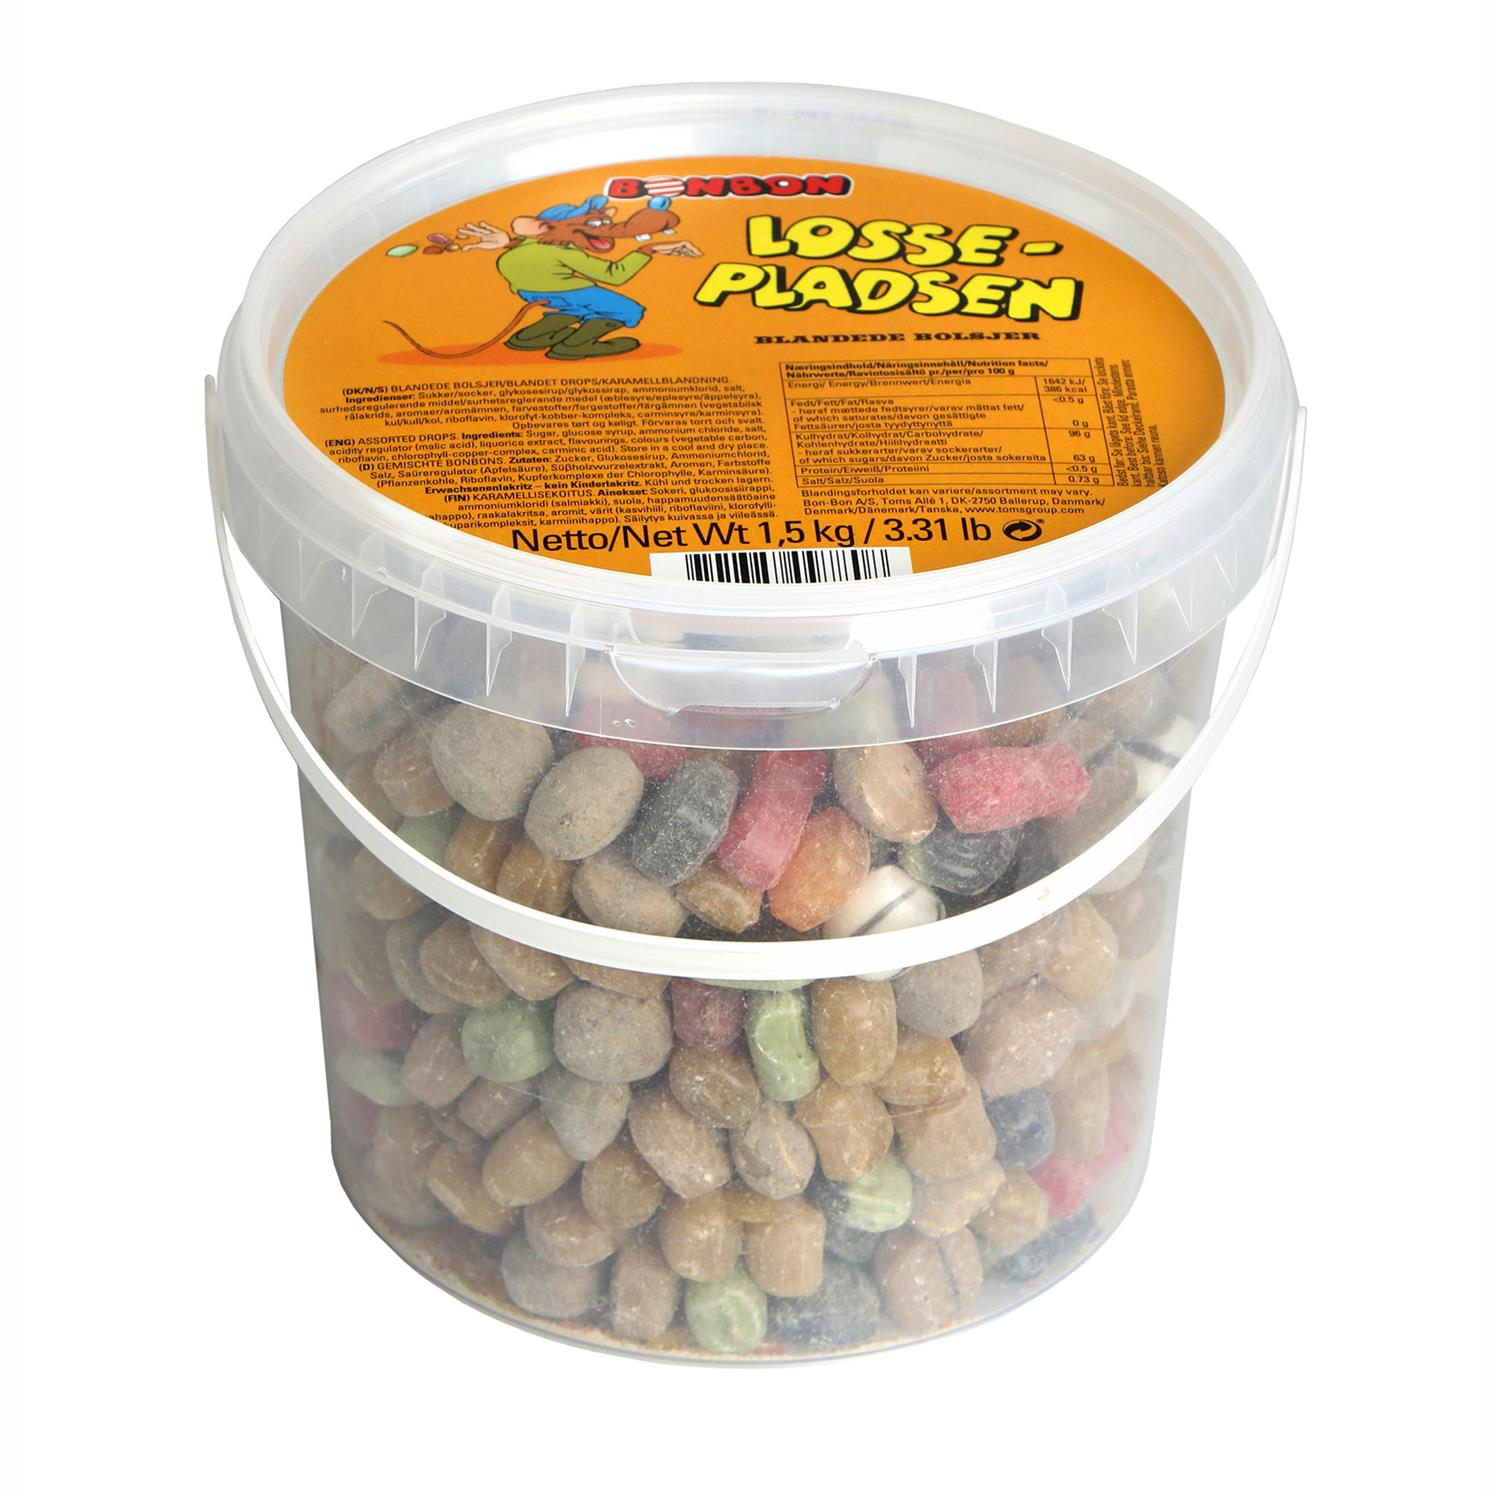
\includegraphics[width=0.4\textwidth]{Billeder/Losseplads.jpg}
	\end{center}
	Producenten af en bestemt type bolscher sælger beholdere á 1500g med bolscher. En grundig stikprøve har vist, at nettovægten af beholderne er normalfordelt med 
	en middelværdi på 1506g og en spredning på 11g. 
\end{opgavetekst}
\begin{delopgave}{(10 point)}{1}
	Afgør, om en beholder med en nettovægt på 1538g er et exceptionelt udfald. 
\end{delopgave}
\begin{meretekst}
	Lad $f$ være tæthedsfunktionen for den stokastiske variabel, der beskriver nettovægten af en beholder med bolscher.
\end{meretekst}
\begin{delopgave}{(10 point)}{2}
	Opskriv et integral, der beskriver sandsynligheden for at få en beholder med en nettovægt på mere end 1510g.
\end{delopgave}

%%%%%%%%%%%%%%%%%%%%%%%%%%%%%%%%%%%%%%%%%%%%%%%%%%%%%%%%%%%%%%%%%%%%%%%
%							Ny Opgave!!!!!							%
%%%%%%%%%%%%%%%%%%%%%%%%%%%%%%%%%%%%%%%%%%%%%%%%%%%%%%%%%%%%%%%%%%%%%%%

\begin{opgavetekst}{Opgave 2}
	En funktion $f:\mathbb{R}^2 \to \mathbb{R}$ er givet ved
	\begin{align*}
		f(x,y) = 2x^2-4x-2y^2+8y.
	\end{align*}
	Funktionen $f$ har netop ét stationært punkt.
\end{opgavetekst}
\begin{delopgave}{(10 point)}{1}
	Bestem det stationære punkt for $f$. 
\end{delopgave}

%%%%%%%%%%%%%%%%%%%%%%%%%%%%%%%%%%%%%%%%%%%%%%%%%%%%%%%%%%%%%%%%%%%%%%%
%							Ny Opgave!!!!!							%
%%%%%%%%%%%%%%%%%%%%%%%%%%%%%%%%%%%%%%%%%%%%%%%%%%%%%%%%%%%%%%%%%%%%%%%

\newpage

\begin{opgavetekst}{Opgave 3}
	En vektorfunktion $\vv{r}:\mathbb{R}\to \mathbb{R}^2$ er givet ved
	\begin{align*}
		\vv{r}(t) = 
		\begin{pmatrix}
			t^2-4 \\
			t^2-6t-3
		\end{pmatrix}.
	\end{align*}
\end{opgavetekst}
\begin{delopgave}{(10 point)}{1}
	Bestem de to skæringspunkter mellem parameterkurven for $\vv{r}$ og $y$-aksen.
\end{delopgave}
\begin{delopgave}{(10 point)}{2}
	Bestem det punkt, hvor parameterkurven for $\vv{r}$ har en vandret tangent. 
\end{delopgave}

%%%%%%%%%%%%%%%%%%%%%%%%%%%%%%%%%%%%%%%%%%%%%%%%%%%%%%%%%%%%%%%%%%%%%%%
%							Ny Opgave!!!!!							%
%%%%%%%%%%%%%%%%%%%%%%%%%%%%%%%%%%%%%%%%%%%%%%%%%%%%%%%%%%%%%%%%%%%%%%%

\begin{opgavetekst}{Opgave 4}
	En funktion $f:\mathbb{R} \to \mathbb{R}$ er givet ved
	\begin{align*}
		f(x) = -\cos(4x^3+13)12x^2.
	\end{align*}
\end{opgavetekst}
\begin{delopgave}{(10 point)}{1}
	Udregn det ubestemte integral $I$ givet ved
	\begin{align*}
		I = \int f(x) dx.
	\end{align*}
\end{delopgave}

%%%%%%%%%%%%%%%%%%%%%%%%%%%%%%%%%%%%%%%%%%%%%%%%%%%%%%%%%%%%%%%%%%%%%%%
%							Ny Opgave!!!!!							%
%%%%%%%%%%%%%%%%%%%%%%%%%%%%%%%%%%%%%%%%%%%%%%%%%%%%%%%%%%%%%%%%%%%%%%%


\begin{opgavetekst}{Opgave 5}
	En funktion $f$ er løsning til differentialligningen
	\begin{align*}
		y' = 30 + 6y
	\end{align*}
\end{opgavetekst}
\begin{delopgave}{(10 point)}{1}
	Bestem en ligning for tangenten til grafen for $f$ gennem punktet $P(1,-4)$.
\end{delopgave}
\begin{delopgave}{(10 point)}{2}
	Bestem den partikulære løsning til differentialligningen, hvis graf skærer gennem punktet $Q(0,-2)$.
\end{delopgave}

%%%%%%%%%%%%%%%%%%%%%%%%%%%%%%%%%%%%%%%%%%%%%%%%%%%%%%%%%%%%%%%%%%%%%%%
%							Ny Opgave!!!!!							%
%%%%%%%%%%%%%%%%%%%%%%%%%%%%%%%%%%%%%%%%%%%%%%%%%%%%%%%%%%%%%%%%%%%%%%%

\end{document}



